\documentclass{article}
\usepackage{listings}
\usepackage{graphicx}
\usepackage{xcolor}
\lstset { %
	language=C++,
	backgroundcolor=\color{black!5}, % set backgroundcolor
	basicstyle=\footnotesize,% basic font setting
}
%opening
\title{C++ Directed Graph Library Tutorial}
\author{}

\begin{document}

    \maketitle

    \tableofcontents
    \newpage
    This tutorial will use an example to help you get started with our graph library. 
    
    \textbf{You'll learn how to:}
    \begin{itemize}
    	\item Create a graph
    	\item Use BFS to find a path in the graph
    	\item Develop a Bellman-Ford Based Shortest Path Algorithms
    \end{itemize}

	\section{What is this Library?}
	This library is a graph and graph algorithms library for C++. Users can easily build a graph and run common graph algorithms like BFS on it. Developers can make use of its api and develop their own graph algorithms. 

    \section {Use our Graph Library}
    First we need to construct a graph. You need to specify the type of vertices and edges in the graph. Here we define two structs: \textit{city} as the vertex type and \textit{dis} as the edge type.
    \begin{lstlisting}
    struct city {
	    string name;
	    city(string input): name(input) {} 
	    string to_string() {
	    	return name;
	    }
    };
    \end{lstlisting}
    
    \begin{lstlisting}
    struct dis {
	    size_t miles;
	    dis(){}
	    dis(size_t input): miles(input) {}
	    string to_string() {
	    	return std::to_string(miles);
	    }
	    const size_t get_val() const{
	    	return miles;
	    }
	    dis operator+(dis d) const{
	    	return dis(miles + d.miles);
	    }
    };
    \end{lstlisting}
    If you want to print out the path you find with our graph algorithms, you need to implement the \textit{to\_string} function for the vertex type.
    \\
    You \textbf{must} implement the \textit{get\_val()} function for the edge type. It should return the weight of the edge. If you want to use any of our path algorithms, you need to implement the operator +.If you want to print out the path you find with our graph algorithms, you need to implement the \textit{to\_string} function.
    Now we will create a graph, representing distances between cities. You can create a graph like this.
    \begin{lstlisting}
    	#include "graph.h"
    
        fixed_directed_dense_graph<city, dis> fddg =
        	fixed_directed_dense_graph<city, dis>(7);
        auto s = fddg.insert_node(city("s"));
        auto t = fddg.insert_node(city("t"));
        auto a = fddg.insert_node(city("a"));
        auto b = fddg.insert_node(city("b"));
        auto c = fddg.insert_node(city("c"));
        auto f = fddg.insert_node(city("f"));
        auto e1 = fddg.insert_edge(s, a, dis(3));
        auto e2 = fddg.insert_edge(s, b, dis(4));
        auto e3 = fddg.insert_edge(a, c, dis(2));
        auto e4 = fddg.insert_edge(a, b, dis(6));
        auto e5 = fddg.insert_edge(a, f, dis(7));
        auto e6 = fddg.insert_edge(b, f, dis(5));
        auto e7 = fddg.insert_edge(c, f, dis(1));
        auto e8 = fddg.insert_edge(c, t, dis(8));
        auto e9 = fddg.insert_edge(f, t, dis(4));
    \end{lstlisting}
The graph looks like this:
\begin{center}
	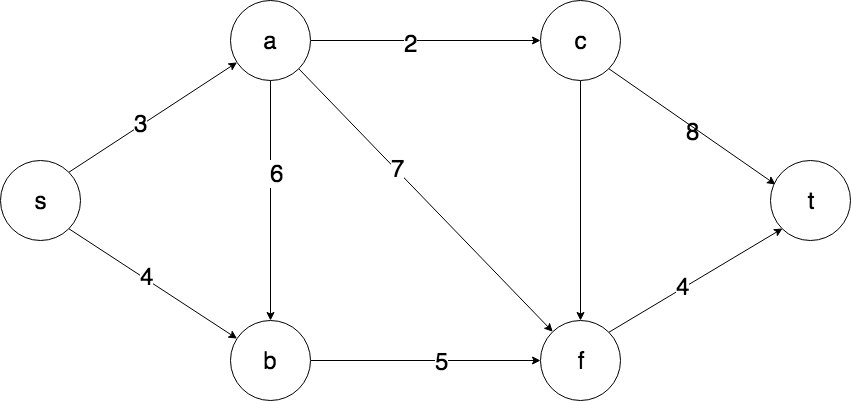
\includegraphics[width=\linewidth]  {graph1.png}
\end{center}
In our library, we provide four types of graphs: Dense Graph, Sparse Graph, Fixed Dense Graph and Fixed Sparse Graph. You can choose one according to your graph. Please refer to our manual for detailed explanation about these graphs. If you use Fixed Dense Graph or Fixed Sparse Graph, you need to pass the number of vertices in the graph as an paremeter when initializing the graph.
\\
To insert a node, simply use the \textit{insert\_node} function. This function will give you a handle, with which you can refer to this node later.
\\
To insert an edge from vertex $u$ to $v$, pass parameters like \textit{(u, v, edge)}. You should pass the handle of $u$ and $v$ instead of the actual vertex type. The last parameter is the edge, it should be the type which you specified when initializing the graph.

    \section {Use our Algorithms}
    You can use the Breadth First Search algorithms like this.
    \begin{lstlisting}
    	#include "algorithms.h"
    	
    	auto bfs_path = bfs_findpath(fddg, s, t);
        bfs_path->print_path();
    \end{lstlisting}
The BFS function will take the graph, the source vertex and the target vertex as the argument. It will return a type \textit{path}. Please refer to our manual for detailed explanation about \textit{path}. Here we simply call its \textit{print\_path()} function to have a look at the path. The output looks like this:

	\begin{lstlisting}
		The path is 
		handle 0
		s to a cost is 3
		handle 2
		a to c cost is 2
		handle 4
		c to t cost is 8
	\end{lstlisting}
Which will give you information about the path we found. It's one of the possible path from $s$ to $t$ in the graph.

	\begin{center}
		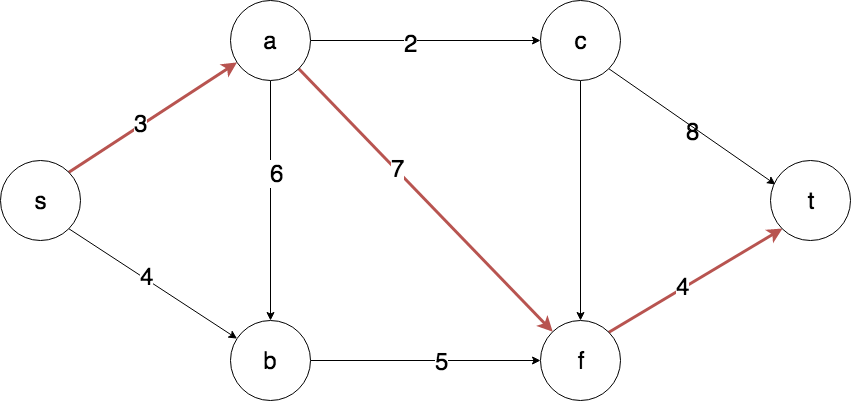
\includegraphics[width=\linewidth]  {graph2.png}
	\end{center}

    \section {Develop your Algorithms}
If you are a developer, you can build your own graph algorithm on top of our library. Here we will show the development of our Single Source Shortest Path algorithm. We use the Bellman-Ford algorithm for implementation.
\begin{lstlisting}
template<typename G>
requires Graph<G>
void shortest_path_bf(G g, typename G::node_handle s,
unordered_map<typename G::node_handle, int>& d,
unordered_map<typename G::node_handle, typename G::node_handle>& pi){
	for (auto v: g.all_nodes()) {
		d[v] = std::numeric_limits<int>::max();
		pi[v] = -1;
	}
	d[s] = 0;

	for (auto v: g.all_nodes()) {
		for (auto v2: g.all_nodes()) {
			for (const auto& e: g.out(v2)) {
				if (d[e.to] > d[v2] + e.info.get_val()){
					d[e.to] = d[v2] + e.info.get_val();
					pi[e.to] = v2;
				}
			}
		}
	}
}
\end{lstlisting}
The implementation is quite straightforward. If you do not know about the Bellman-Ford Algorithm, you can have a look at www.columbia.edu/~cs2035/courses/csor4231.F17/sp.pdf. The pseudocode on slide 6 and 9 can give you an understanding of the algorithm. Here we omit the part of checking negative loop in the pseudocode.
\\
First we need to initialize the map $d$ and $pi(\pi)$ to store the cost and the previous vertex at any vertex. Then we need to do a loop for $|V|$ times. This can be easily done by calling the \textit{all\_nodes()} function on the graph. It will give you handles of all nodes in the graph. The next step is to traverse all edges in the graph. You can do this by combining looping \textit{all\_nodes()} and \textit{out()}. \textit{out(v)} will give you edges from vertex $v$ to other vertices. By traversing all out edges on every vertex, you go through evert edge in the graph exactly one time.
\\
Thanks to the sufficient api in the library, you can implement your own graph algorithm simply like translating pseudocode to C++ code.

\section{Celebrate!}
Celebrate!
By completing this tutorial, you’ve learned to use our graph library!

Here’s what you accomplished in this tutorial:

    \begin{itemize}
	\item Create a graph
	\item Use BFS to find a path in the graph
	\item Develop a Bellman-Ford Based Shortest Path Algorithms
\end{itemize}

To learn more about our library, we recommend reading the manual. You might also visit our GitHub repository and have a look at the source code at https://github.com/streammy2013/cpp-graph-library. Do not hesitate to contact us if you have any thoughts about the library!
\end{document}
